\subsection{Streams}

\definition{CUDA Streams} are \textbf{sequences of operations} (like kernel launches or memory copies) \textbf{that execute in order}. By \emph{default}, all \textbf{operations in CUDA run in the default stream}, which is \emph{blocking} and \emph{sequential}.

\highspace
Is important to understand the CUDA streams, because by changing the default order, we can gain performance:
\begin{itemize}
    \item Concurrency. By using multiple streams, we can \textbf{perform operations in parallel}, leading to better performance.
    \item Overlap Computation and Data Transfer. For example, \textbf{while one\break stream is running a kernel on the GPU}, \textbf{another stream can be copying data to or from the GPU}.
\end{itemize}

\highspace
\begin{flushleft}
    \textcolor{Green3}{\faIcon{balance-scale} \textbf{Default vs Non-Default Streams}}
\end{flushleft}
\begin{itemize}
    \item Default Stream:
    \begin{itemize}
        \item Executes operations \textbf{sequentially}.
        \item \textbf{Blocks all other streams} until its operations are complete.
    \end{itemize}

    \item Non-Default Streams:
    \begin{itemize}
        \item Allow for \textbf{concurrent} execution of operations.
        \item Operations within the \textbf{same stream execute sequentially}, but \textbf{operations in different streams can run in parallel}.
    \end{itemize}
\end{itemize}

\highspace
\begin{flushleft}
    \textcolor{Green3}{\faIcon{tools} \textbf{CUDA implementation}}
\end{flushleft}
\begin{enumerate}
    \item \textbf{Creating Streams}. We can create streams using \texttt{cudaStreamCreate}.
    \begin{lstlisting}[language=C++]
cudaStream_t stream1, stream2;
cudaStreamCreate(&stream1);
cudaStreamCreate(&stream2);\end{lstlisting}

    \item \textbf{Launching Kernels in Streams}. Launch kernels in different streams to execute them concurrently.
    \begin{lstlisting}[language=C++]
// Launching a kernel in stream1
kernel1<<<blocks, threads, 0, stream1>>>(...);

// Launching a kernel in stream2
kernel2<<<blocks, threads, 0, stream2>>>(...);\end{lstlisting}

    \newpage

    \item \textbf{Synchronizing Streams}. We can synchronize individual streams or all streams.
    \begin{lstlisting}[language=C++]
// sync specific stream:
cudaStreamSynchronize(stream1);

// sync all streams
cudaDeviceSynchronize();\end{lstlisting}

    \item \textbf{Destroying Streams}. Once we're done with the streams, it's important to destroy them to free up resources.
    \begin{lstlisting}[language=C++]
cudaStreamDestroy(stream1);
cudaStreamDestroy(stream2);\end{lstlisting}
\end{enumerate}

\begin{examplebox}
    Imagine we have two kernels to execute, \texttt{kernel1} and \texttt{kernel2}. If we use the default stream, they will execute one after the other:
    \begin{enumerate}
        \item Launch \texttt{kernel1};
        \item Wait for \texttt{kernel1} to complete;
        \item Launch \texttt{kernel2};
        \item Wait for \texttt{kernel2} to complete.
    \end{enumerate}

    This sequential execution means the GPU is not fully utilized.

    Using two non-default streams, we can launch both kernels to execute concurrently:

    \begin{enumerate}
        \item Create two streams:
        \begin{lstlisting}[language=C++]
cudaStream_t stream1, stream2;
cudaStreamCreate(&stream1);
cudaStreamCreate(&stream2);\end{lstlisting}

        \item Launch \texttt{kernel1} in \texttt{stream1} and \texttt{kernel2} in \texttt{stream2}:
        \begin{lstlisting}[language=C++]
kernel1<<<blocks, threads, 0, stream1>>>(...);
kernel2<<<blocks, threads, 0, stream2>>>(...);\end{lstlisting}
    \end{enumerate}

    Now, \texttt{kernel1} and \texttt{kernel2} can run in parallel, allowing the GPU to be used more efficiently.
\end{examplebox}

\newpage

\begin{examplebox}[: DAG]
    The following image shows a series of tasks (\texttt{A1} through \texttt{A8}) organized in a DAG. The arrows between tasks indicate dependencies, meaning one task must complete before another can start.
    \begin{itemize}
        \item Default Stream: contains tasks \texttt{A0}, and \texttt{A8}.
        \item Non-Default Streams: there are three non-default streams that contain tasks \texttt{A1}, \texttt{A4}, \texttt{A6}, \texttt{A2}, \texttt{A5}, \texttt{A7}, and \texttt{A3}.
    \end{itemize}
    \begin{center}
        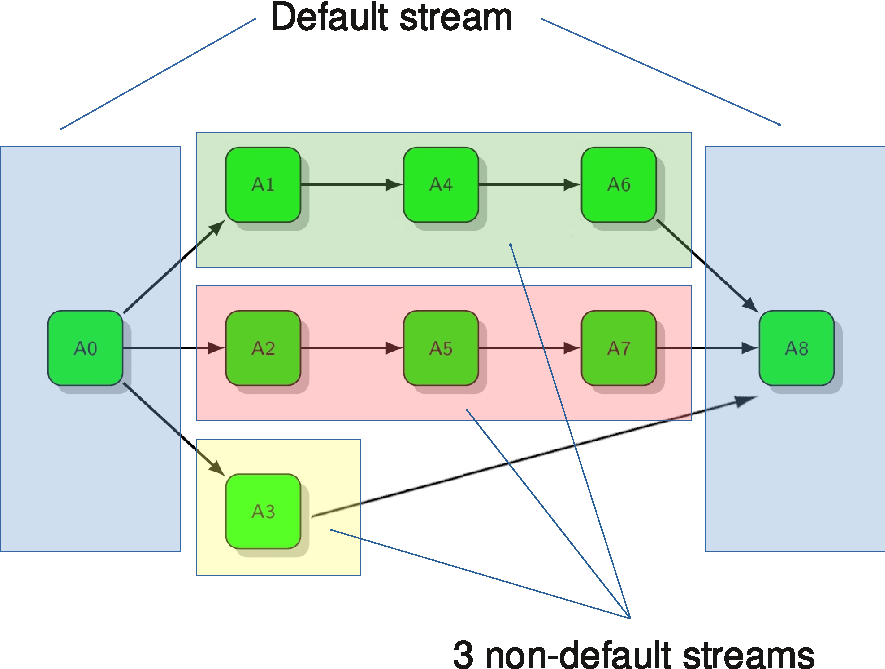
\includegraphics[width=.8\textwidth]{img/cuda-stream-dag-1.pdf}
    \end{center}

    The execution flow is:
    \begin{itemize}
        \item Initial Tasks.
        \begin{itemize}
            \item Task \texttt{A0} starts in the default stream.
            \item Concurrently, tasks \texttt{A1}, \texttt{A2}, and \texttt{A3} run in non-default streams (\texttt{stream1}, \texttt{stream2}, and \texttt{stream3}).
        \end{itemize}
        \item Dependent Tasks.
        \begin{itemize}
            \item After \texttt{A1}, \texttt{A2}, and \texttt{A3} complete, \texttt{A4}, \texttt{A5}, \texttt{A6}, and \texttt{A7} start in the respective non-default streams.
        \end{itemize}
        \item Final Task.
        \begin{itemize}
            \item After all dependent tasks are complete, task \texttt{A8} runs in the default stream.
        \end{itemize}
    \end{itemize}

    The implementation is the following:
    \begin{enumerate}
        \item Task \texttt{A0} in Default Stream.
        \begin{lstlisting}[language=C++]
kernelA0<<<blocks, threads>>>(...); // Default stream\end{lstlisting}

        \newpage

        \item Tasks \texttt{A1}, \texttt{A2}, and \texttt{A3} in Different Streams:
        \begin{lstlisting}[language=C++]
// Stream 1
kernelA1<<<blocks, threads, 0, stream1>>>(...);
// Stream 2
kernelA2<<<blocks, threads, 0, stream2>>>(...);
// Stream 3
kernelA3<<<blocks, threads, 0, stream3>>>(...);\end{lstlisting}
     
        \item Synchronize Streams Before Dependent Tasks:
        \begin{lstlisting}[language=C++]
cudaStreamSynchronize(stream1);
cudaStreamSynchronize(stream2);
cudaStreamSynchronize(stream3);\end{lstlisting}

        \item Tasks \texttt{A4}, \texttt{A5}, \texttt{A6}, and \texttt{A7} in Non-Default Streams:
        \begin{lstlisting}[language=C++]
// Stream 1
kernelA4<<<blocks, threads, 0, stream1>>>(...);
// Stream 2
kernelA5<<<blocks, threads, 0, stream2>>>(...);
// Stream 1
kernelA6<<<blocks, threads, 0, stream1>>>(...);
// Stream 2
kernelA7<<<blocks, threads, 0, stream2>>>(...);\end{lstlisting}

        \item Synchronize Streams Again Before Final Task:
        \begin{lstlisting}[language=C++]
cudaStreamSynchronize(stream1);
cudaStreamSynchronize(stream2);
cudaStreamSynchronize(stream3);\end{lstlisting}

        \item Task A8 in Default Stream:
        \begin{lstlisting}[language=C++]
kernelA8<<<blocks, threads>>>(...); // Default stream\end{lstlisting}

        \item Destroying Streams:
        \begin{lstlisting}[language=C++]
cudaStreamDestroy(stream1);
cudaStreamDestroy(stream2);
cudaStreamDestroy(stream3);\end{lstlisting}
    \end{enumerate}
\end{examplebox}

\noindent
Using concurrent CUDA streams helps manage complex task dependencies in DAG-like applications. By running independent tasks in different streams, we can achieve parallel execution and optimize the performance of our CUDA applications. The example shows how to create streams, start kernels in these streams, synchronize them, and finally destroy the streams to free up resources. Finally, \textbf{non-default streams and manual memory management allow for overlapping data transfers and computations}.
